\chapter{Data and Resources}
\label{dataresources}

\section{Data}
\label{data}
The data for this study was derived from the Temple University Hospital's EEG corpus which includes over $30\text{,}000$ EEGs spanning the years from $2002$ to the present as described and provided by \citet{tuhwebsite}. The original data consists of raw European Data Format (EDF+\nomenclature{EDF+}{European Data Format}) files, a format commonly used for exchanging and storing multichannel biological and physical signals, and the corresponding labels for each of these files in LBL files. Both EDF files and the LBL files were stored in session folders with a single patient's data and doctors' notes on that patient's EEGs. There are a total of $339$ folders labeled from \verb+session1+ to \verb+session339+. The label files are interpretable by Temple University's publicly available Python script \cite{tuhwebsite}, which transforms the label files into a readable format.  Each channel is annotated as pertaining to one of six classes as described in \cref{tab:classes} with a granularity of one second. We assume that the data provided to us was time aligned correctly with the labels. For more details on the dataset see \citet{tuh}

% All of these labels are of interest for our purposes since the purpose of this project is to learn a low-dimensional representation which may lead to more meaning when looking at EEG signals

\begin{table}[!ht]
	\captionsetup[table]{skip=10pt}
	\centering
	\caption[Set of classes]{Set of classes for the TUH EEG Corpus. After consulting \citet{harati2015improved}, it was determined that BCKG, ARTF and EYBL are noise-like signals, and the rest are all seizure-like signals, i.e. indications of common events that occur in seizures. }
	\begin{tabular}{rL{5.5cm}}
		\toprule
		Codename & Description                                  \\ \midrule
		BCKG     & Background noise                             \\
		ARTF     & Artifacts                                    \\
		EYBL     & Eyeball movement                             \\
		SPSW     & Spikes and sharp waves                       \\
		PLED     & Periodic lateralized epileptiform discharges \\
		GPED     & Generalized periodic epileptiform discharges \\\bottomrule
	\end{tabular}
	\label{tab:classes}
\end{table}


The EDF files contain raw signals with different channels from electrodesplaced in the standard $10$-$20$ system and were decoded using Python's MNE package. A total of $22$ montages were found in each label file. The power spectral density (PSD\nomenclature{PSD}{Power Spectral Density}) plot of the signal was visualized using the \verb+RawEDF.plot_psd()+ function. The bandwidth of the signals was between $0$ Hz to around $130$ Hz. It was revealed that the signals contained power line noise at $60$ Hz and $120$ Hz as seen in the sample PSD plot in \cref{fig:psd}. 

\begin{figure}[!ht]
	\centering
	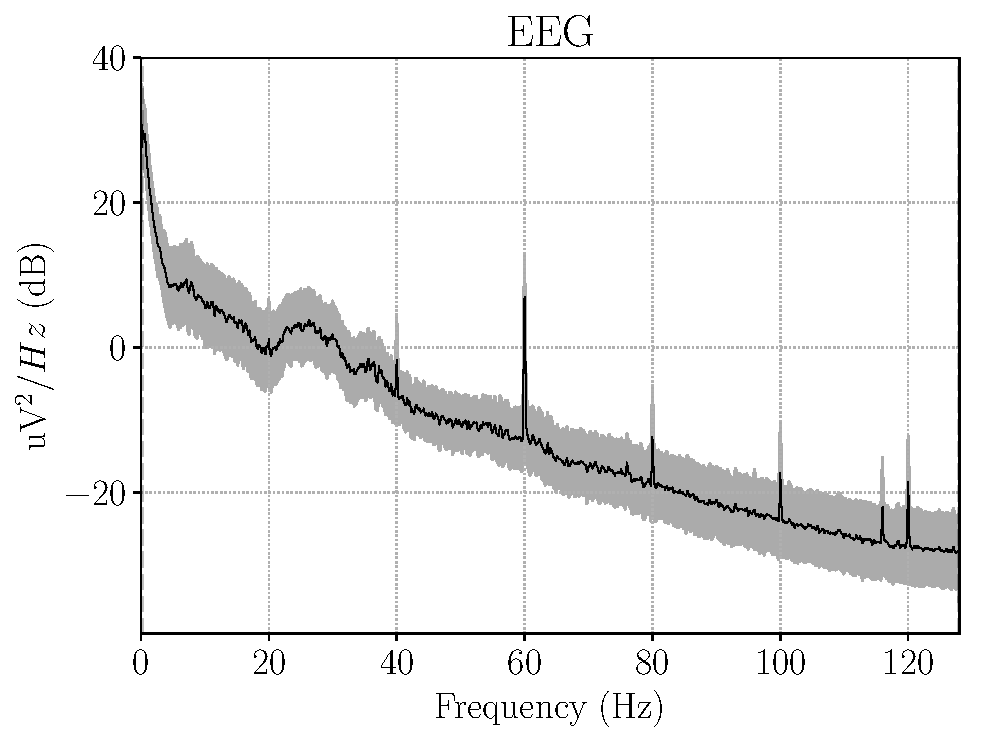
\includegraphics[height=0.45\linewidth]{pictures/psd.pdf}
	\caption[Power Spectral Density Plot of Raw Signals]{Power spectral density plot of raw signals using the MNE packagel}\label{fig:psd}  
\end{figure}

Hence, we apply notch filters at $60$ Hz and $120$ Hz to remove power line noise, and a bandpass filter with a $1$ Hz to $70$ Hz pass-band to remove any high-frequency noise as the bulk of the signal power was within this band. We apply the Short-Term Fourier Transform (STFT\nomenclature{STFT}{Short Term Fourier Transform}) provided by the MNE package with a window of $140$ samples and a stride of two samples which results in the spectrogram represented as a $71 \times 125$ tensor for each one-second window of the signal as shown in \cref{fig:stft}. 

\begin{figure}[!ht]
	\centering
	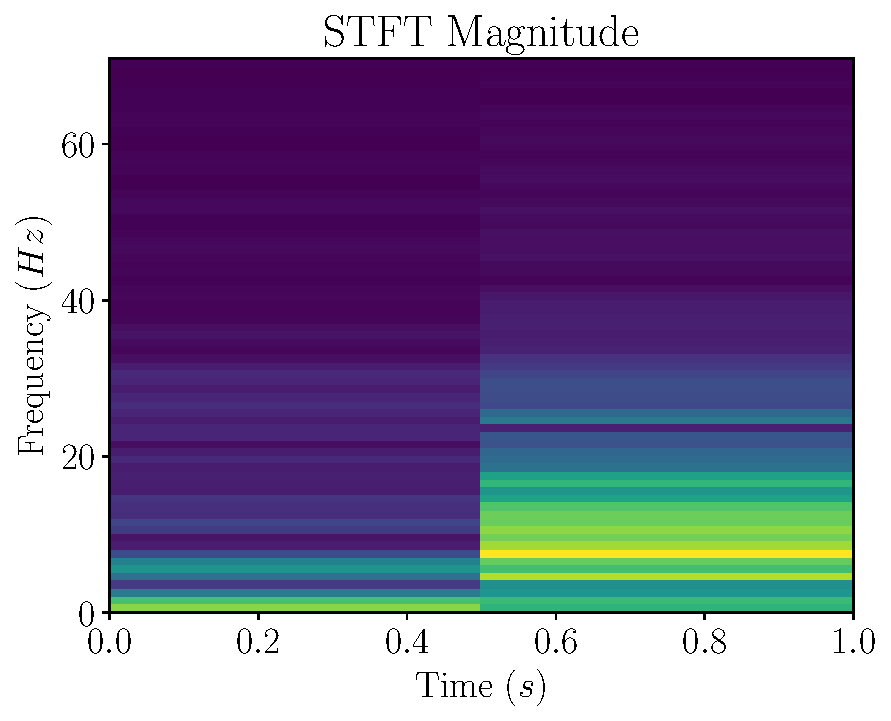
\includegraphics[height=0.45\linewidth]{pictures/plot21.pdf}
	\caption[Example of Spectrogram]{Spectrogram of a second of notch and bandpass filtered signal}\label{fig:stft}  
\end{figure}

Additionally, we globally normalize the signal power in order to standardize the input to the system that we designed and only use the real part of the spectrogram data. The raw time-domain data was not utilized in this experiment because the literature \cite{eegs_info, eeg_info2, mayo_eegs} on EEGs indicated that the frequency domain is what contains data that is useful for our purpose.

% Of course, recurrent neural networks may use been helpful in deciphering this information from the time domain itself, however, it is generally known that they are relatively harder to train and was by-passed. 

We did not use the spatial information implicitly provided to us by the $10$-$20$ system's spatial structure. This decision was made because the resulting tensor would have become a $22 \times 71 \times 125$ tensor of values and the amount of time taken to process this tensor would have been longer than the time taken to process a $71 \times 125$ tensor. Furthermore, even if it were computationally possible for us to process the larger tensor for each second of signal, there was no possible way to consistently label the tensor as each montage was labeled independently of the others. Hence, there was no possible way to consistently label all $22$ montages with a single label. As a result, we only used a single channel's input as opposed to all $22$ channels' inputs. 

We also realized that the dataset is highly imbalanced. More than $80\%$ of the data was labeled as noise-like signals. Since we were looking for anomalies in the dataset, it was necessary to use stratified sampling to help compensate for this imbalance which may result in a high accuracy. We split the $71 \times 125$ tensors into mutually exclusive training and validation sets. Each set is disjoint in both patient and sample acquisition, i.e. no single patient appears in both sets and no two windows from a single acquisition appear in both sets. We follow an $85/15\%$ split for the training/validation set. Due to the large nature of the training set in this situation and the impossibility of training on every triplet possible, a random set of triplets were selected for each training iteration. 

\section{Resources}


\subsection*{Tensorflow}

Tensorflow and TF-Slim, as described by \citet{tensorflow} and \citet{tfslim},  are frameworks which provided a way to build scalable, computational graphs for machine learning. Tensorflow's use of automatic differentiation, as described by \citet{autodiff}, allowed for precise calculations of gradients for networks without error due to floating-point errors. Furthermore, automatic differentiation also helped in this project since the loss function depended on multiple example data points, i.e. the anchor, the positive and the negative,  as opposed to a single example data point. TF-Slim's implementation of commonly used computational graph layers (e.g. convolutional layers) helped us define the network without explicitly defining and coding weight matrices. 

\subsection*{SciKit Learn}
SciKit Learn is a Python module developed by \citet{sklearn} that provided implementations of common machine learning algorithms and some commonly used accessory functions. In particular, it provided us the k-NN algorithm used throughout the paper to classify validation signals, the confusion matrix calculation function used to analyze our validation results, and the t-SNE reduction algorithm used to analyze the high dimesional latent space in a reduced, 2-dimensional space. SciKit Learn was also built with NumPy and matplotlib, and was easily compatible with the rest of our source code. 

\subsection*{MNE Package}

The MNE package is a Python module developed by \citet{mne} that provided implementations for manipulating biological signal data. It has functions necessary to read, analyze, filter and convert raw data in EDF files to NumPy arrays. These functions allowed us to refine the data instead of processing the raw, time-domain signal.